\documentclass[12pt, fleqn]{article}
\usepackage{../../../template/template}
\usepackage{../../../template/fortickets}

%сам документ
\begin{document}
\begin{center}
  \huge Практика по геометрии

  \Large (преподаватель Амрани И. М.)

  \large Записал Костин П.А.
\end{center}

Данный документ неидеальный, прошу сообщать о найденных недочетах в \href{https://vk.com/drab_existence_a}{вконтакте}
\tableofcontents
\newpage

\section{(03.09.2019) Кривые и поверхности}
\begin{Example}
    \[\gamma: \R \ra \R^3,\q \gamma \in C^2,\text{ т.ч.}\q |\gamma(t)|=1\ \forall t \in \R\]
    \[\text{Д-ть, что } \gamma'(t) \bot \gamma''(t)\ \forall t \in \R\]
\end{Example}

\begin{Proof}
    \[|\gamma'|=1 \lra \sqrt{<\dot{\gamma},\dot{\gamma}>}=1 \lra <\dot{\gamma},\dot{\gamma}>=1\]
    \[(<\dot{\gamma},\dot{\gamma}>)'=(1)' \Ra 2<\dot{\gamma},\ddot{\gamma}> = 0\]
    Вообще очевидно, но если нет, то:
    \[(<\dot{\gamma},\dot{\gamma}>)'=(\sum_{i=1}^3 \dot{\gamma_i}^2)' = \sum_{i=1}^3 2 \dot{\gamma_i} \ddot{\gamma_i} = 2<\dot{\gamma},\ddot{\gamma}>\]
\end{Proof}

\begin{Example}
    \[\gamma: \R \ra \R^3,\q \gamma \in C^3,\q |\gamma'|=1,\q \gamma'' \neq 0\]
    \[T(t)=\gamma'(t),\q B(t)=T(t) \times N(t),\q N(t)=\frac{\gamma''(t)}{|\gamma''(t)|}\]
    \begin{enumerate}
      \item Д-ть, что $\{T(t), N(t),B(t) \}$ - ОНБ
      \item Найти координаты $\dfrac{dT}{dt}$, $\dfrac{dN}{dt}$, $\dfrac{dB}{dt}$ в базисе $\{T,N,B\}$
    \end{enumerate}
\end{Example}

\begin{sol}
  \begin{enumerate}
    \item Очевидно, $B(t) = \us{=1}{T} \cdot \us{=1}{N} \sin \angle (T,N)$
    \[T \bot N \ (\text{по пред. задаче}),\q B \bot N,\q B \bot T\ (\text{по опр. вект. произв.})\]

    \item По определению "взятием производной"\,получаем:
    \[\dfrac{dT}{dt} = 0T + |\ddot{\gamma}|N + 0B\]
    \[<N, T> = 0 \Ra <\frac{d N}{dt}, T> + <N, \frac{d T}{dt}> = 0\]
    \[\text{Аналогично } 0 = <\frac{d T}{dt},B> = - <\frac{d B}{dt}, T>\]
    \[|\ddot{\gamma}| = <\frac{d N}{dt}, T> = -<N, \frac{d T}{dt}>\]
    \[\frac{d N}{dt} = -|\ddot{\gamma}|T + 0N + \tau(t)B\]
    \[\frac{d B}{dt} = 0T - \tau(t)N + 0B\]
  \end{enumerate}
\end{sol}
\section{(10.09.2019) Задачи на кривые}
Мы хотим найти $\tau$ через $\dot{\gamma},\ \ddot{\gamma},\ \dddot{\gamma}$
\begin{remark}
  На плоскоти в каждой точке гладкой кривой есть окружность, которая наилучшим образом приближает кривую
  \[R=\frac{1}{|\ddot{\gamma}|},\q |\ddot{\gamma}| := \ae \text{ - кривизна}\]
  \begin{figure}[h]
	    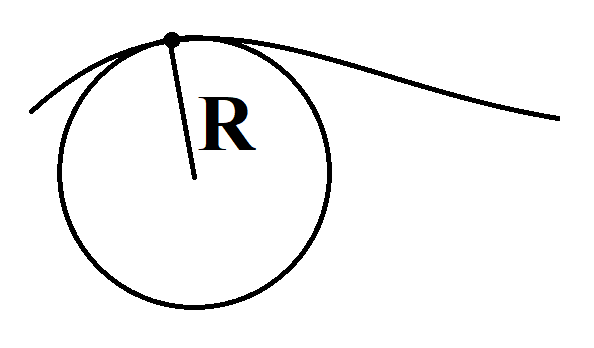
\includegraphics[scale=0.3]{pics/2_1.png}
	    \centering
	\end{figure}
\end{remark}
\begin{Sol} [продолжение]
  \[\tau = <\frac{d N}{dt},\ B>\]
  \[\frac{d N}{dt} = \Br{\frac{\ddot{\gamma}}{\abs{\ddot{\gamma}}}}' = \frac{\dddot{\gamma} |\ddot{\gamma}| - |\ddot{\gamma}|' \ddot{\gamma}}{|\ddot{\gamma}|^2}\]
  \begin{multline*}
    \Ra <\frac{d N}{dt},\ B>=<\frac{\dddot{\gamma} |\ddot{\gamma}| - |\ddot{\gamma}|' \ddot{\gamma}}{|\ddot{\gamma}|^2},\ \frac{\dot{\gamma} \times \ddot{\gamma}}{|\ddot{\gamma}|}> = \\
    \qq \qq = \frac{1}{|\ddot{\gamma}|^3} <\dddot{\gamma} |\ddot{\gamma}|-|\ddot{\gamma}|' \ddot{\gamma},\ \dot{\gamma} \times \ddot{\gamma}> \us{\text{см. на N}}{=} \\
    = \frac{1}{|\ddot{\gamma}|^3} <\dddot{\gamma} |\ddot{\gamma}|,\ \dot{\gamma} \times \ddot{\gamma}> = \frac{1}{|\ddot{\gamma}|^2} <\dddot{\gamma},\ \dot{\gamma} \times \ddot{\gamma} > = \frac{(\dot{\gamma},\ \ddot{\gamma},\ \dddot{\gamma})}{|\ddot{\gamma}|^2}
  \end{multline*}
\end{Sol}

\begin{Example}
  \[\gamma: \R \ra \R^3,\q t \mapsto (4 \cos(t),\ 5-5 \sin(t),\ -3\cos(t))\]
  \begin{enumerate}
    \item Найти $\ae$ и $\tau$
    \item Понять, что из себя представляет линия
  \end{enumerate}
\end{Example}

\begin{sol}
  \begin{enumerate}
    \item Предыдущую задачу мы не можем просто так применить, потому что $|\dot{\gamma}|=5 \neq 1$, но мы можем перепараметризовать:
    \[\w{\gamma}: \R \ra \R^3,\q t \mapsto (4 \cos(\frac{t}{5}),\ 5-5 \sin(\frac{t}{5}),\ -3\cos(\frac{t}{5}))\]
    \[\w{\dot{\gamma}} = (-\frac{4}{5} \sin(\frac{t}{5}),\ -\cos(\frac{t}{5}),\ \frac{3}{5} \sin(\frac{t}{5}))\]
    \[\Ra |\w{\dot{\gamma}}|=1\]
    \[\w{\ddot{\gamma}} = (-\frac{4}{25} \cos(\frac{t}{5}),\ \frac{1}{5} \sin(\frac{t}{5}),\ \frac{3}{25} \cos(\frac{t}{5}))\]
    \[\Ra \ae = |\w{\ddot{\gamma}}| = \frac{1}{25}\]
    \[\w{\dddot{\gamma}} = (\frac{4}{125} \sin(\frac{t}{5}),\ \frac{1}{25} \cos(\frac{t}{5}),\ -\frac{3}{125} \sin(\frac{t}{5}))\]
    \[\Ra \tau = \frac{(\dot{\gamma},\ \ddot{\gamma},\ \dddot{\gamma})}{|\ddot{\gamma}|^2}=25 (\dot{\gamma},\ \ddot{\gamma},\ \dddot{\gamma})=0\]
    \item Наша линия находится на плоскости:
    \[3x+0y+4z\]
    И лежит на сфере:
    \[x^2+(y-5)^2+z^2=25\]
    Значит она представляет из себя окружность, потому что есть разные точки
    \begin{figure}[H]
  	    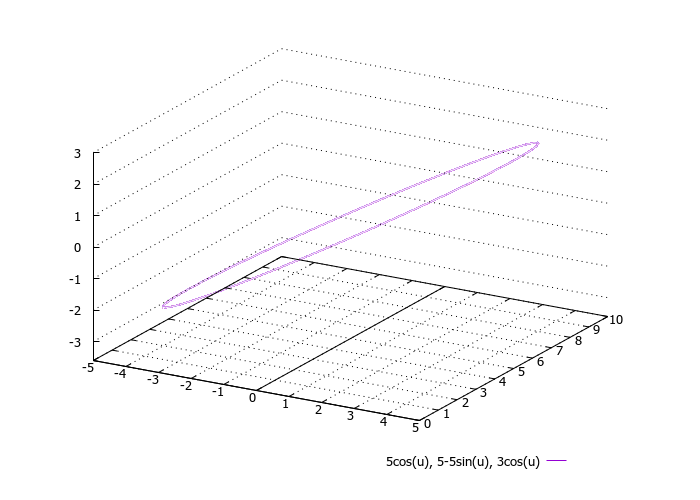
\includegraphics[scale=0.6]{pics/2_2.png}
  	    \centering
  	\end{figure}
  \end{enumerate}
\end{sol}

\begin{Example}
  \[\gamma: \R \ra \R^3,\q t \mapsto (\cos(t),\ \sin(t),\ t)\]
  \begin{enumerate}
    \item Построить график
    \begin{figure}[H]
  	    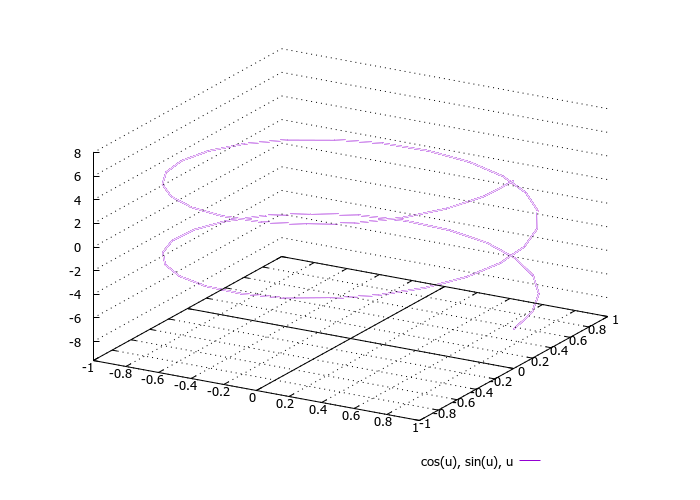
\includegraphics[scale=0.6]{pics/2_3.png}
  	    \centering
  	\end{figure}
    \item Найти $\ae$ и $\tau$
  \end{enumerate}
\end{Example}

\begin{sol}
    Аналогично $t \ra \dfrac{t}{\sqrt{2}}$
    \[\w{\gamma}: \R \ra \R^3,\q t \mapsto (\cos(\frac{t}{\sqrt{2}}),\ \sin(\frac{t}{\sqrt{2}}),\ \frac{t}{\sqrt{2}})\]
    \[\w{\dot{\gamma}}=(-\frac{1}{\sqrt{2}} \sin(\frac{t}{\sqrt{2}}),\ \frac{1}{\sqrt{2}} \cos(\frac{t}{\sqrt{2}}),\ \frac{1}{\sqrt{2}})\]
    \[\Ra |\w{\dot{\gamma}}|=1\]
    \[\w{\ddot{\gamma}}=(-\frac{1}{2} \cos(\frac{t}{\sqrt{2}}),\ -\frac{1}{2} \sin(\frac{t}{\sqrt{2}}),\ 0)\]
    \[\Ra \ae = |\w{\ddot{\gamma}}| = \frac{1}{2}\]
    \[\w{\dddot{\gamma}}=(\frac{1}{2 \sqrt{2}} \sin(\frac{t}{\sqrt{2}}),\ -\frac{1}{2 \sqrt{2}} \cos(\frac{t}{\sqrt{2}}),\ 0)\]
    \[\tau = \frac{(\dot{\gamma},\ \ddot{\gamma},\ \dddot{\gamma})}{|\ddot{\gamma}|^2}\]
    \[(\dot{\gamma},\ \ddot{\gamma},\ \dddot{\gamma}) = \det
    \begin{pmatrix}
      -\frac{1}{\sqrt{2}} \sin(\frac{t}{\sqrt{2}}) & \frac{1}{\sqrt{2}} \cos(\frac{t}{\sqrt{2}}) & \frac{1}{\sqrt{2}}\\ \\
      -\frac{1}{2} \cos(\frac{t}{\sqrt{2}}) & -\frac{1}{2} \sin(\frac{t}{\sqrt{2}}) & 0\\ \\
      \frac{1}{2 \sqrt{2}} \sin(\frac{t}{\sqrt{2}}) & -\frac{1}{2 \sqrt{2}} \cos(\frac{t}{\sqrt{2}}) & 0
    \end{pmatrix} = \frac{1}{8}\]
\end{sol}

\section{(17.09.2019) Поверхности}
\begin{Example}
  \[\gamma: \R \ra \R^3, \q t \mapsto (r(t),\ 0,\ z(t)),\text{ где $r: \R \ra \R$, $z: \R \ra \R$}\]
  Найти параметрищацию поверхности вращения вокруг $OZ$
\end{Example}

\begin{proof}
  Из геометрических соображений: $(r(t) \cos \varphi,\ r(t)\sin \varphi,\ z(t)),\ \varphi \in [0,\ 2\pi]$\\
  Более строго:
  \[\begin{pmatrix}
    \cos \alpha & -\sin \alpha & 0\\
    \sin \alpha & \cos \alpha & 0\\
    0 & 0 & 1
  \end{pmatrix}
  \begin{pmatrix}
    r(t)\\
    0\\
    z(t)
  \end{pmatrix}
  =
  \begin{pmatrix}
    r(t) \cos \alpha\\
    r(t) \sin \alpha\\
    z(t)
  \end{pmatrix}\]
\end{proof}

\begin{definition}
  Гладкая двухмерная поверхность:
  \[F: \os{\text{откр}}{\us{t,\ s}{U}} \subset \R^2 \ra \R^3\]
  т.ч. $\dfrac{\d F}{\d S}$, $\dfrac{\d F}{\d t}$ - непрерывные функции
\end{definition}

\begin{definition}
  Гладкая регулярная поверхность:
  \[F: \os{\text{откр}}{\us{t,\ s}{U}} \subset \R^2 \ra \R^3\]
  т.ч. $\dfrac{\d F}{\d S}$, $\dfrac{\d F}{\d t}$ - линейно независимы\\
  "регулярная = скорость не обнуляется"
\end{definition}
\begin{figure}[H]
    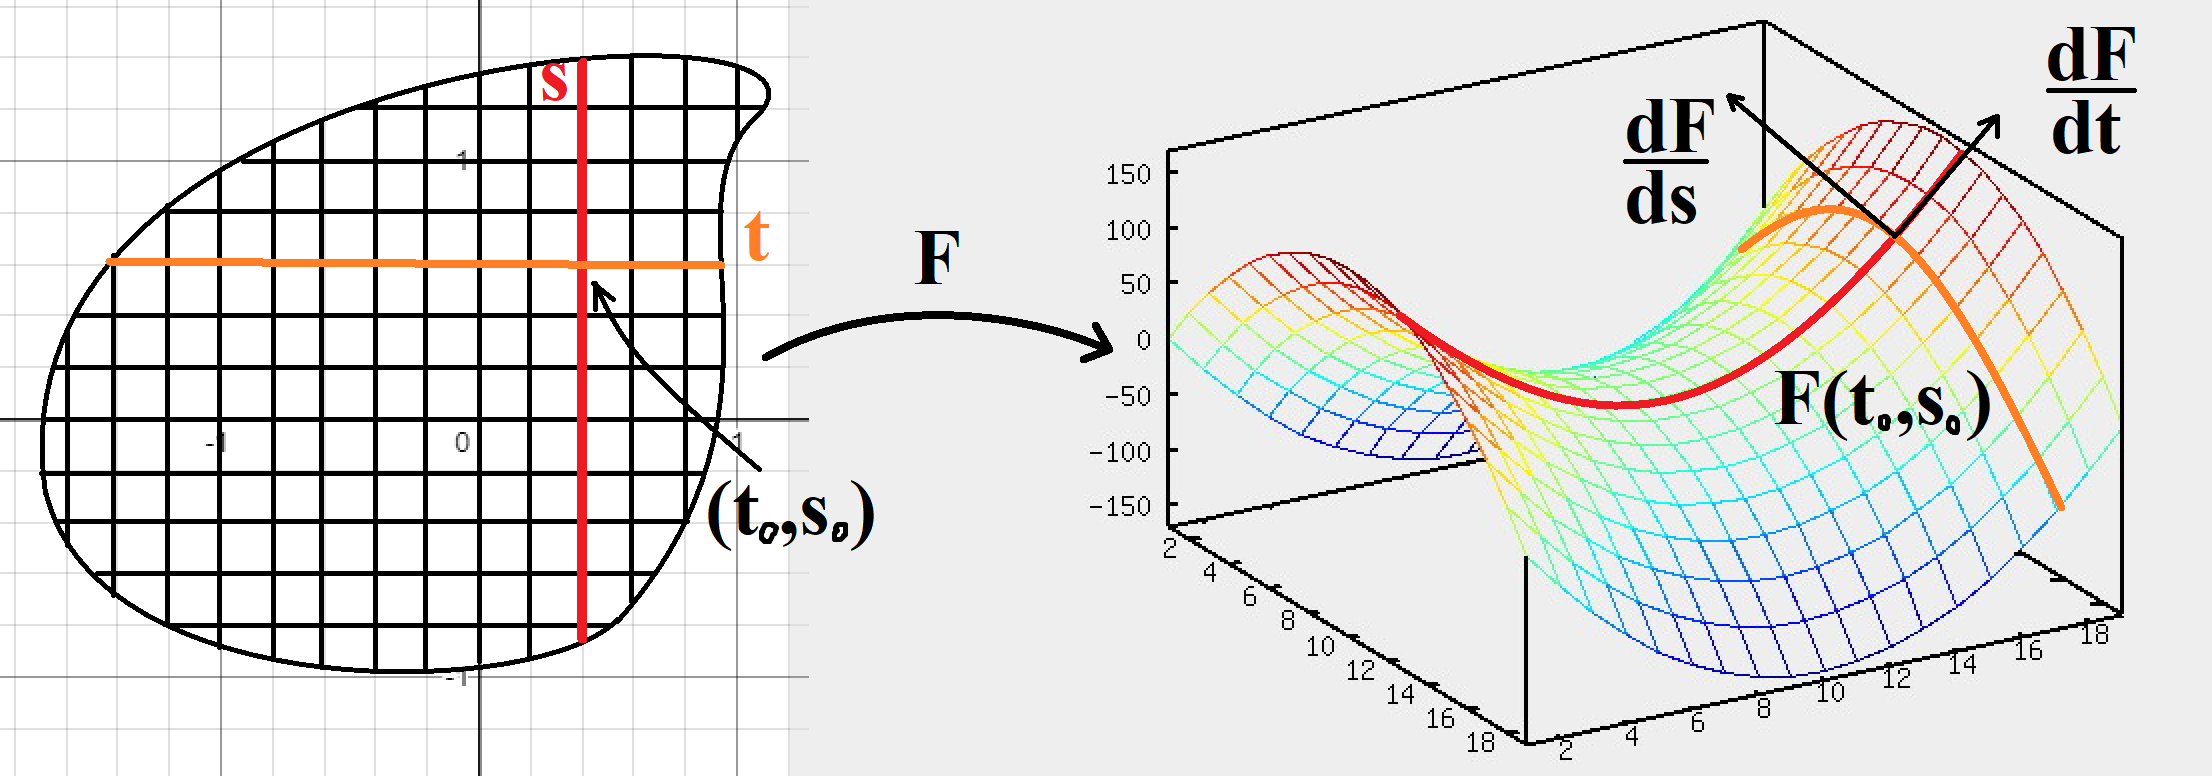
\includegraphics[scale=0.2]{pics/3_1.png}
    \centering
\end{figure}

\section{(24.10.2019) Первая фундаментальная форма}
\begin{Example}
  \[F: U \subset \R^2 \ra \R^3\]
  \begin{multline*}
    $\det \begin{pmatrix}
      <\dfrac{\d F}{\d t}, \dfrac{\d F}{\d t}> & <\dfrac{\d F}{\d s}, \dfrac{\d F}{\d t}>\\
      \\
      <\dfrac{\d F}{\d t}, \dfrac{\d F}{\d s}> & <\dfrac{\d F}{\d s}, \dfrac{\d F}{\d s}>
    \end{pmatrix} = \\ \\
      = <\frac{\d F}{\d t}, \frac{\d F}{\d t}> <\frac{\d F}{\d s}, \frac{\d F}{\d s}> - <\frac{\d F}{\d s}, \frac{\d F}{\d t}> <\frac{\d F}{\d t}, \dfrac{\d F}{\d s}> =\\ \\
     =\abs{\dfrac{\d F}{\d t}}^2 \abs{\dfrac{\d F}{\d s}}^2 - \abs{\dfrac{\d F}{\d s}}^2 \abs{\dfrac{\d F}{\d t}}^2 \cos^2 t = \abs{\dfrac{\d F}{\d t}}^2 \abs{\dfrac{\d F}{\d s}}^2
    =
    \begin{vmatrix}
      \dfrac{\d F}{\d t} \times \dfrac{\d F}{\d s}
    \end{vmatrix}^2$
  \end{multline*}
\end{Example}

\begin{Remark}
  \[A(S)=\sum A(\square)\]
  \[A(\square) \approx \abs{\dfrac{\d F}{\d t} \times \dfrac{\d F}{\d s}} \Delta t \Delta s\]
  \[\RNumb{1}(F)= \begin{pmatrix}
    <\dfrac{\d F}{\d t}, \dfrac{\d F}{\d t}> & <\dfrac{\d F}{\d s}, \dfrac{\d F}{\d t}>\\
    \\
    <\dfrac{\d F}{\d t}, \dfrac{\d F}{\d s}> & <\dfrac{\d F}{\d s}, \dfrac{\d F}{\d s}>
  \end{pmatrix}\]
  \[A(S)= \iint \abs{\dfrac{\d F}{\d t} \times \dfrac{\d F}{\d v}} dt ds = \iint \sqrt{\det \RNumb{1}(F)} dt ds\]
\end{Remark}

\begin{Example}
  \[F: (0,\ 2\pi) \times (0,\ 2\pi) \ra \R^3\]
  \[(\theta,\ \varphi) \ra (\cos \theta \sin \varphi,\ \cos \theta \cos \varphi,\ \sin \theta)\]
  \begin{enumerate}
    \item Доказать, что образ F находится на сфере радиуса 1
    \item Найти S сферы через $\RNumb{1}(F)$
  \end{enumerate}
\end{Example}

\begin{proof}
  \begin{enumerate}
    \item Видно из параметрического уравнения сферы что это сфера, а также понятен радиус и её центр
    \[\begin{cases}
      x = x_0 + R \cdot \sin \theta\cdot \cos \phi,\\
      y = y_0 + R \cdot \sin \theta\cdot \sin \phi,\\
      z = z_0 + R \cdot \cos \theta,\\
    \end{cases}\]
    где $\theta \in [0, \pi]$ и $\phi \in [0, 2\pi)$ (у нас будет сдвиг на угол)
    \item Найдем переменные для $\RNumb{1}(F)$:
    \[<\frac{\d F}{\d \theta},\ \frac{\d F}{\d \theta}> = \sin^2 \theta \sin^2 \varphi + \sin^2 \theta \cos^2 \varphi + \cos^2 \theta = 1\]
    \[<\frac{\d F}{\d \theta},\ \frac{\d F}{\d \varphi}> = 0,\q <\frac{\d F}{\d \varphi},\ \frac{\d F}{\d \theta}> = 0,\q <\frac{\d F}{\d \varphi},\ \frac{\d F}{\d \varphi}> = \cos^2 \theta\]
    \[\Ra \RNumb{1}(F)=\begin{pmatrix}
      1 & 0\\
      0 & \cos^2 \theta
    \end{pmatrix}\]
    \[\Ra A(S) = \iint \sqrt{\det \RNumb{1}(F)} d\theta d\varphi = \int_0^\pi \int_0^{2\pi} |\cos \theta|d\theta d\varphi = \int_0^\pi 4 d\varphi = 4 \pi\]
  \end{enumerate}
\end{proof}

\section{(01.10.2019) Ещё задача на $\RNumb{1}(F)$}

\begin{Example}
  \[F: U \subset \R^2 \ra \R^3,\q C^1 \text{ регулярная}\]
  \begin{figure}[H]
      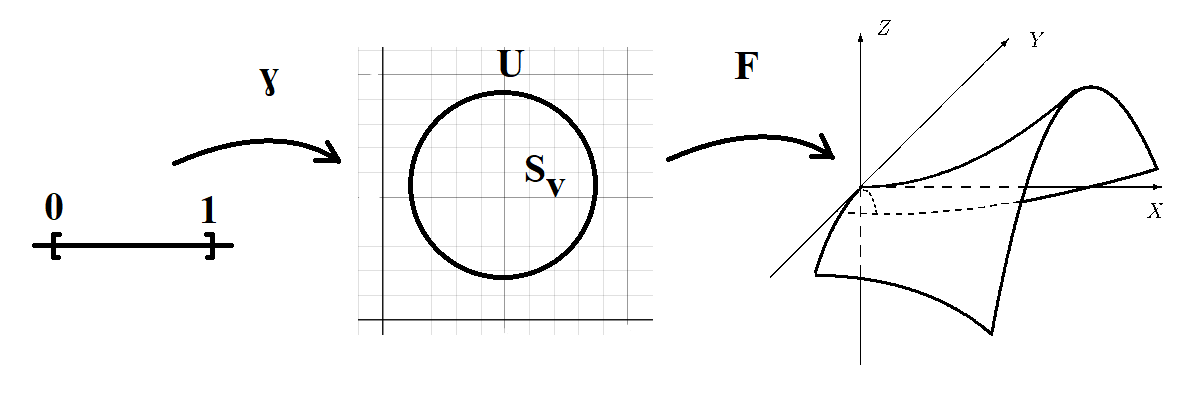
\includegraphics[scale=0.4]{pics/4_1.png}
      \centering
  \end{figure}
  Найти длину $\w{\gamma} = F \circ \gamma$ через $\gamma$ и $\RNumb{1}(F)$
\end{Example}

\begin{Sol}
  \[l(F \circ \gamma) := \int_0^1 |F \circ \gamma(t)'| dt\]
  \[\frac{d(F \circ \gamma(t))}{dt} = \ub{\text{вектор}}{\frac{\d F}{\d x}} \ob{\text{скаляр}}{\dot{\gamma_1}(t)}+\frac{\d F}{\d y} \dot{\gamma}_2(t)=\]
  \[=<\frac{\d F}{\d x}\dot{\gamma_1}(t)+\frac{\d F}{\d y} \dot{\gamma}_2(t),\ \frac{\d F}{\d x}\dot{\gamma_1}(t)+\frac{\d F}{\d y} \dot{\gamma}_2(t)>=\]
  \[=<\frac{\d F}{\d x}, \frac{\d F}{\d x}> \dot{\gamma_1^2}(t) + 2<\frac{\d F}{\d x}, \frac{\d F}{\d y}> \dot{\gamma_1}(t)\dot{\gamma_2}(t) + <\frac{\d F}{\d y}, \frac{\d F}{\d y}> \dot{\gamma_2^2}(t)=\]
  \[= (\dot{\gamma_1}, \dot{\gamma_2}) \RNumb{1}(F) \begin{pmatrix}
    \dot{\gamma_1}\\ \dot{\gamma_2}
  \end{pmatrix}\]
  \[\Ra l(F \circ \gamma) = \int_0^1 \sqrt{(\dot{\gamma_1}, \dot{\gamma_2}) \RNumb{1}(F) \begin{pmatrix}
    \dot{\gamma_1}\\ \dot{\gamma_2}
  \end{pmatrix}} dt\]
\end{Sol}

\section{(01.10.2019) Вторая фундаментальная форма}

\begin{Definition}
  \[F: \us{x,y}{U} \subset \R^2 \ra \R^3 \qq C^2 \text{ регулярная}\]
  \[|\frac{\d F}{\d x} \times \frac{\d F}{\d y}| \neq 0\]
  \[n:=\dfrac{\dfrac{\d F}{\d x} \times \dfrac{\d F}{\d y}}{|\dfrac{\d F}{\d x} \times \dfrac{\d F}{\d y}|} \text{ - перп. обоим и по модулю 1}\]
  \[L=<\frac{\d^2 F}{\d x^2},\ n>,\q M=<\frac{\d^2 F}{\d x \d y},\ n>,\q N=<\frac{\d^2 F}{\d y^2},\ n>\]
  \[\RNumb{2}(F) = \begin{pmatrix}
    L & M\\
    M & N
  \end{pmatrix}\]
\end{Definition}

\begin{Remark}
  \[\RNumb{2}(F) \text{ говорит, какая ПВП лучше всего приближает в данной точке}\]
\end{Remark}

\begin{example}
  Пусть есть сфера радиуса r:
  \[\begin{cases}
    x = x_0 + R \cdot \sin \theta\cdot \cos \phi,\\
    y = y_0 + R \cdot \sin \theta\cdot \sin \phi,\\
    z = z_0 + R \cdot \cos \theta,\\
  \end{cases}\]
  где $\theta \in [-\dfrac{\pi}{2},\ \dfrac{\pi}{2}]$ и $\phi \in [0,\ 2\pi)$\\
  Найти $\RNumb{2}(F)$, $\RNumb{1}(F)$ и $\dfrac{\det(\RNumb{2})}{\det(\RNumb{1})}$
\end{example}

\begin{sol}
  Посчитаем $\RNumb{1}(F)$:
  \[\frac{\d F}{\d \theta} = (-r \sin\theta \cos\varphi,\ -r \sin\theta \sin\varphi,\ r \cos\theta)\]
  \[\frac{\d F}{\d \varphi} = (-r \cos\theta \sin\varphi,\ r \cos\theta \cos\varphi,\ 0)\]
  \[<\frac{\d F}{\d \theta}, \frac{\d F}{\d \theta}> = r^2,\q
  <\frac{\d F}{\d \theta}, \frac{\d F}{\d \varphi}> = 0\]
  \[<\frac{\d F}{\d \varphi}, \frac{\d F}{\d \theta}> = 0,\q
  <\frac{\d F}{\d \varphi}, \frac{\d F}{\d \varphi}> = r^2 \cos^2 \theta\]
  \[\Ra \RNumb{1}(F) =
  \begin{pmatrix}
    r^2 & 0\\
    0 & r^2 \cos^2 \theta
  \end{pmatrix}\]
  Посчитаем $\RNumb{2}(F)$:
  \[\frac{\d^2 F}{\d \theta^2} = (-r \cos \varphi \cos\theta,\ -r \cos\theta \sin\varphi,\ -r \sin\theta)\]
  \[\frac{\d^2 F}{\d \theta \d\varphi} = (r \sin \theta \sin\varphi,\ -r \sin\theta \cos\varphi,\ 0)\]
  \[\frac{\d^2 F}{\d \varphi^2} = (-r \cos \theta \cos\varphi,\ -r \cos\theta \sin\varphi,\ 0)\]
  \begin{Reminder}
    В правом ортонормированном базисе:\\
    Если два вектора $\vec{a}$ и $\vec{b}$ представлены координатами
    \[\vec{a} = (a_x,\ a_y,\ a_z),\q \vec{b} = (b_x,\ b_y,\ b_z),\]
    то их векторное произведение имеет координаты
    \[[a,\ \vec{b}] = (a_y b_z - a_z b_y,\ a_z b_x - a_x b_z,\ a_x b_y - a_y b_x)\]
    Для запоминания этой формулы удобно использовать мнемонический определитель:
    \[[a,\ \vec{b}] =
    \begin{vmatrix}
      \mathbf i & \mathbf j & \mathbf k \\
      a_x & a_y & a_z \\
      b_x & b_y & b_z
    \end{vmatrix},\]
    где $\mathbf i = (1, 0, 0)$, $\mathbf j = (0, 1, 0)$, $\mathbf k = (0, 0, 1)$
  \end{Reminder}
  \[\frac{\d F}{\d \teta} \times \frac{\d F}{\d \varphi} = (-r^2 \cos^2 \theta \cos\varphi,\ -r^2 \cos^2 \theta \sin\varphi,\ -r^2 \sin \theta \cos \theta)\]
  \[\abs{\frac{\d F}{\d \teta} \times \frac{\d F}{\d \varphi}} = \r^2 \cos\theta]\]
  \[n = \dfrac{\dfrac{\d F}{\d \teta} \times \dfrac{\d F}{\d \varphi}}{\abs{\dfrac{\d F}{\d \teta} \times \dfrac{\d F}{\d \varphi}}} = (- \cos\theta \cos\varphi,\ -\cos\theta \sin\varphi, -\sin\theta)\]
  \[L = <\frac{\d^2 F}{\d \theta^2},\ \ol{n}> = r\]
  \[M = <\frac{\d^2 F}{\d \theta \d \varphi},\ \ol{n}> = 0\]
  \[N = <\frac{\d^2 F}{\d \varphi^2},\ \ol{n}> = r \cos^2 \theta\]
  \[\Ra \RNumb{2}(F) =
  \begin{pmatrix}
    r & 0\\
    0 & r \cos^2 \theta
  \end{pmatrix}\]
  \[K = \frac{\det \RNumb{2}(F)}{\det \RNumb{1}(F)} = \frac{1}{r^2} \text{ - кривизна Гаусса}\]
\end{sol}

\begin{example}
  Пусть $\gamma: t \ra (t - \th(t),\ 0,\ \dfrac{1}{\ch(t)}),\q t>0$
  \begin{enumerate}
    \item Найти S поверхности, полученной вращением $\gamma$ вокруг $OZ$
    \item Найти $\RNumb{2}(F)$, $\RNumb{1}(F)$ и $K=\dfrac{\det(\RNumb{2})}{\det(\RNumb{1})}$
    \item Площадь $S_F$
  \end{enumerate}
\end{example}

\begin{Sol}

\end{Sol}

\end{document}
